\documentclass[onecolumn]{article}
%\usepackage{url}
%\usepackage{algorithmic}
\usepackage[a4paper]{geometry}
\usepackage{datetime}
\usepackage[margin=2em, font=small,labelfont=it]{caption}
\usepackage{graphicx}
\usepackage{mathpazo} % use palatino
\usepackage[scaled]{helvet} % helvetica
\usepackage{microtype}
\usepackage{amsmath}
\usepackage{subfigure}
% Letterspacing macros
\newcommand{\spacecaps}[1]{\textls[200]{\MakeUppercase{#1}}}
\newcommand{\spacesc}[1]{\textls[50]{\textsc{\MakeLowercase{#1}}}}

\title{\spacecaps{Final Report : Logistic Regression }\\ \normalsize \spacesc{CENG 3521 , DATA MINING} }

\author{Cansel Hatice Küçükyılmaz-Aynur Salman\\canselhky@gmail.com – salmanaynur20@gmail.com}

%\date{\today\\\currenttime}
\date{\today}

\begin{document}
\maketitle

\begin{abstract}
In this project, chemicals and disease, which is a real data set, was cleaned and logistic regression analysis was performed using this cleared data set. As a result of the project, it was seen whether the chemicals had an effect on the diseases. Visualizations were used to make the result clearer.
\end{abstract}


\section{Introduction}
Nowadays, chemicals have an important place in our lives, especially with drugs, and they increase your quality of life significantly. In our project, using the data set showing the relationship between chemicals and drugs, it was examined whether the drug has a chemical relationship.Logistic regression analysis, a supervised learning classification method, was used to examine this relationship. Classification is a field of supervised machine learning that tries to predict which class or category some assets belong to based on their characteristics. A classification type called binary or binomial classification was used. The dependent variable is  called the target variable. Because  of the target dimension were looking at was a categorical data that can be represented as a binary. In general binary representation, the two results of the response variable "success" and "failure" and represent them with 1 (for success) and 0 (for failure).
\section{Preprocessing of Data}
This section should describe what work was done and how, specifically how you solved the different tasks. For this type of lab report it can be beneficial to put each assignment in its own subsection.

\subsection{OverView of dataset}

 The dataset provides the chemical directly contributed to the disease information. It includes 5610 records and 21 fields. Dataset includes chemical names, disease name, verify relationship, diseases id. (Table 1.1)
 \begin{figure}[h!t]
\centering
    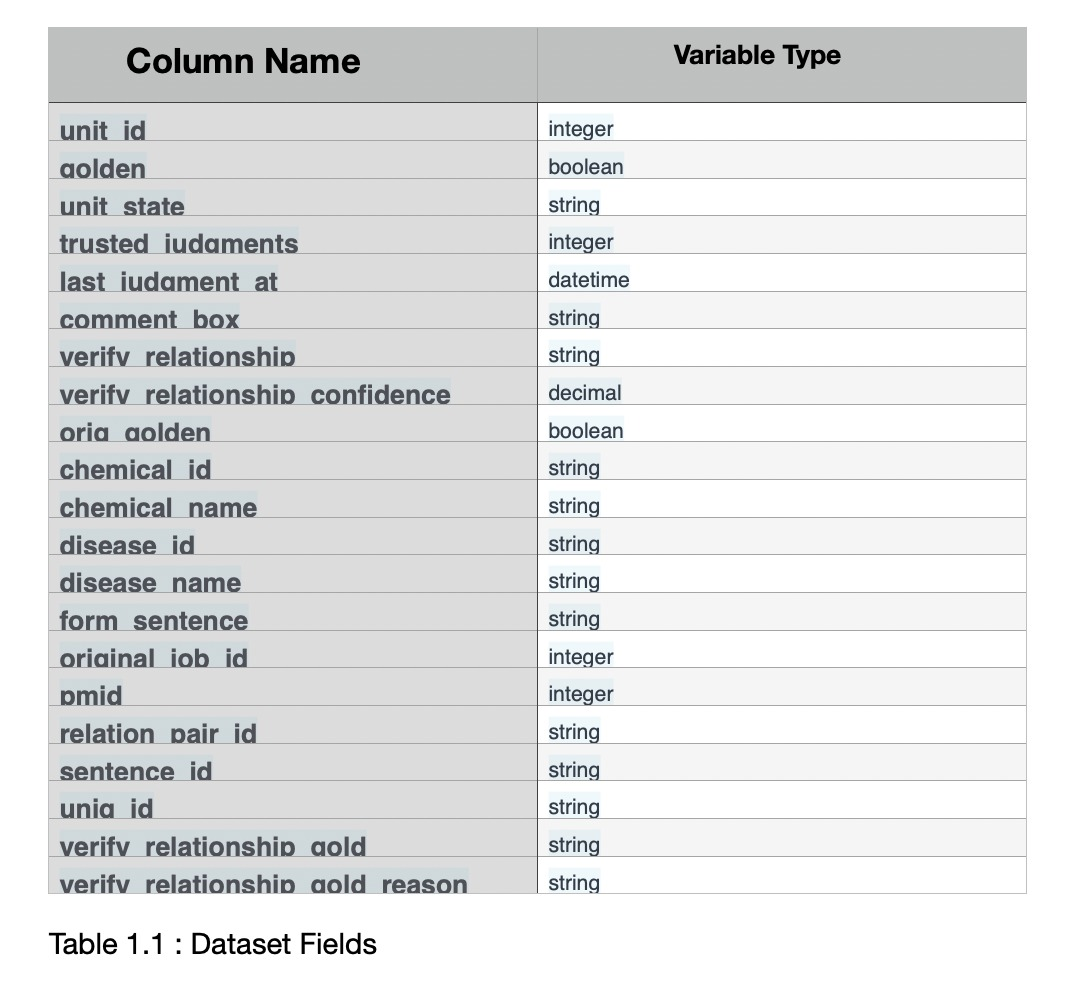
\includegraphics[width=.6\linewidth]{fig/dataset.jpeg}
\caption{\label{fig:dataset}
Dataset Fields}
\end{figure}.
 
 The original dataset is available from :  https://data.world/crowdflower/chems-contributing-to-disease/workspace/data-dictionary

\subsection{Read Dataset}
The csv file was read using pandas library and converted to  Pandas’ dataframe. Using the empty method of the board, it was checked whether the dataframe was loaded or not, and it was observed that it was loaded correctly.
\subsection{Info Dataset}
Using the info method, the data types in the created dataframe and the number of data they contain were displayed.

\subsection{Drop Null Data}
By loading the missingno package in python, the null data in each column in the dataframe was visualized (Figure 2.1), and as a result, the columns that do not directly affect the classification to be made were removed from the dataset using pandas’ dropna method. And as a result, it was seen that there is no null value in the dataset (Figure 2.2).
\begin{figure}[h!t]
\centering
\subfigure[Before Drop Null Data]{\centering
    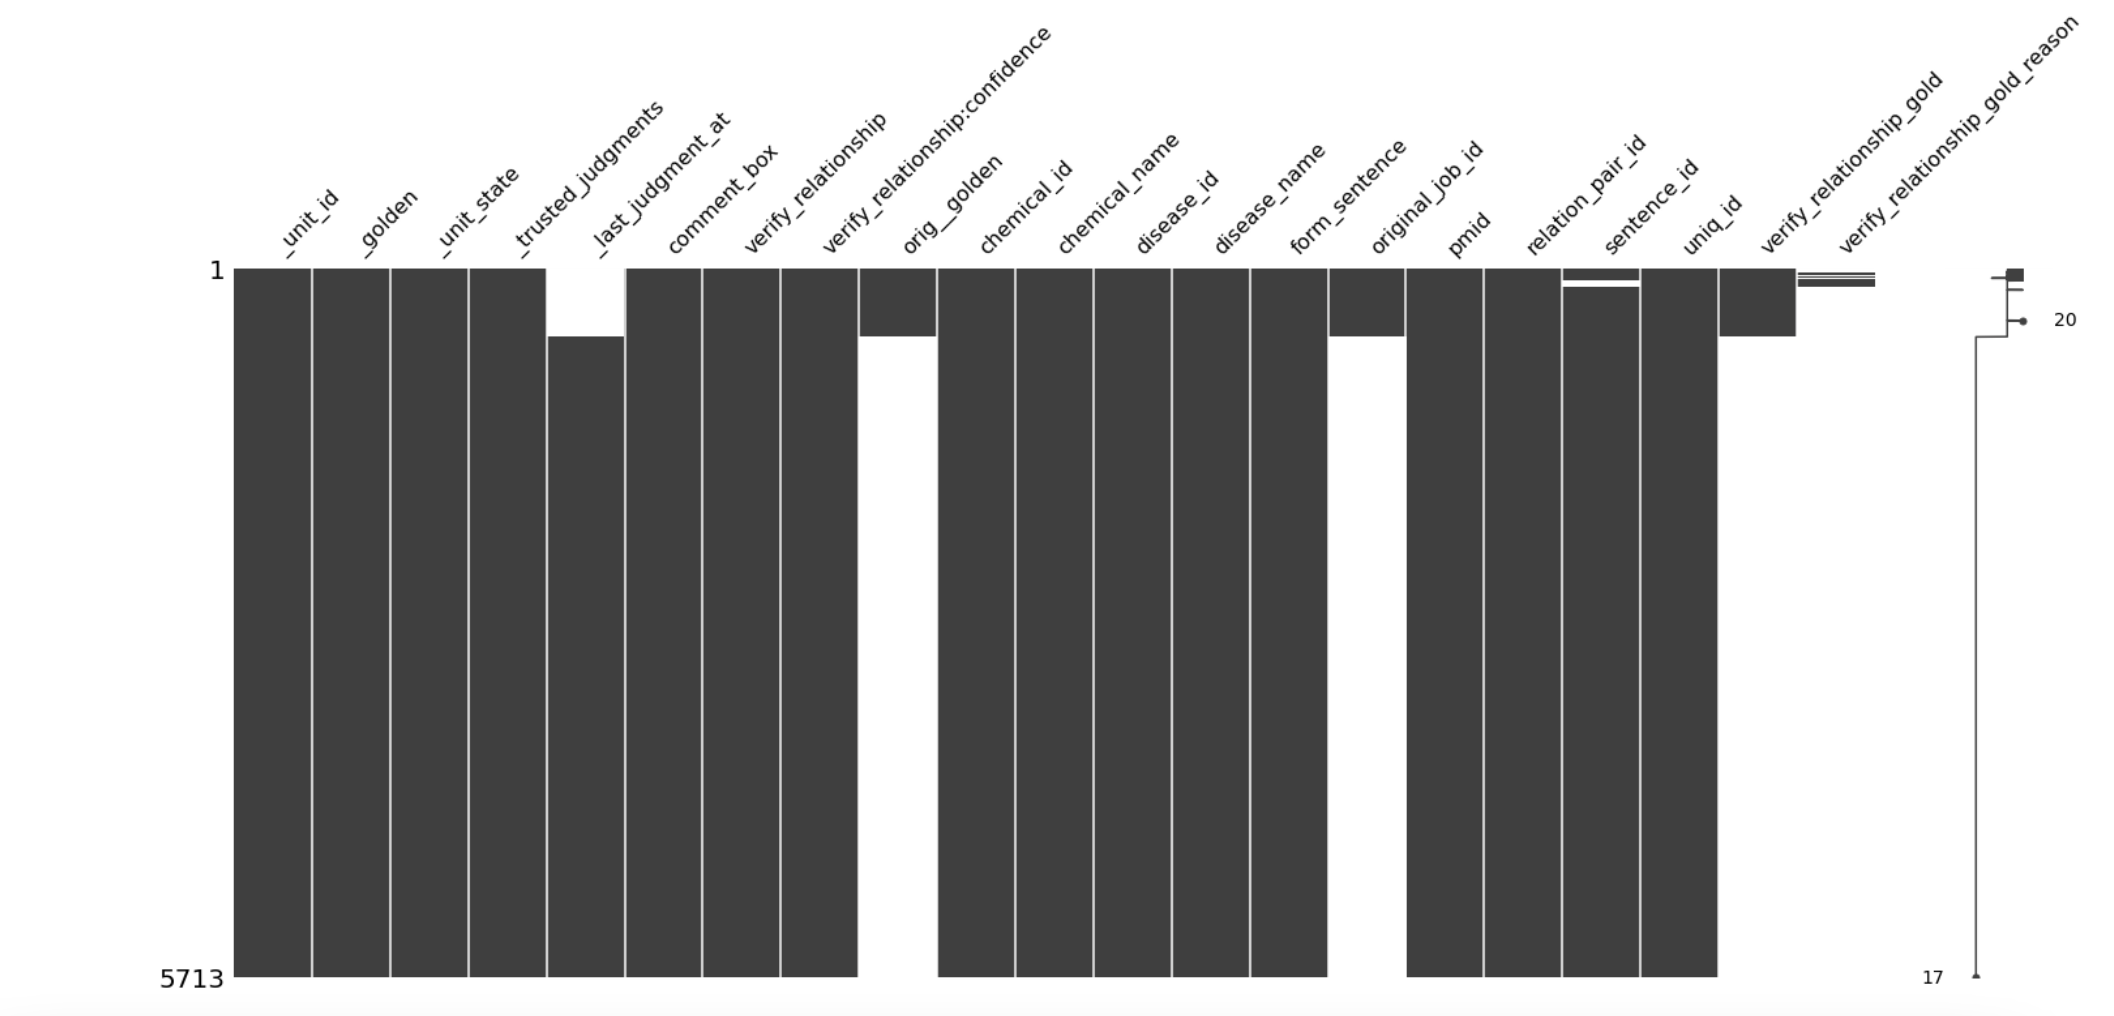
\includegraphics[width=.5\linewidth]{fig/data.png}
        \label{fig:demo-standard}}
\subfigure[After Drop Null Data]{\centering
    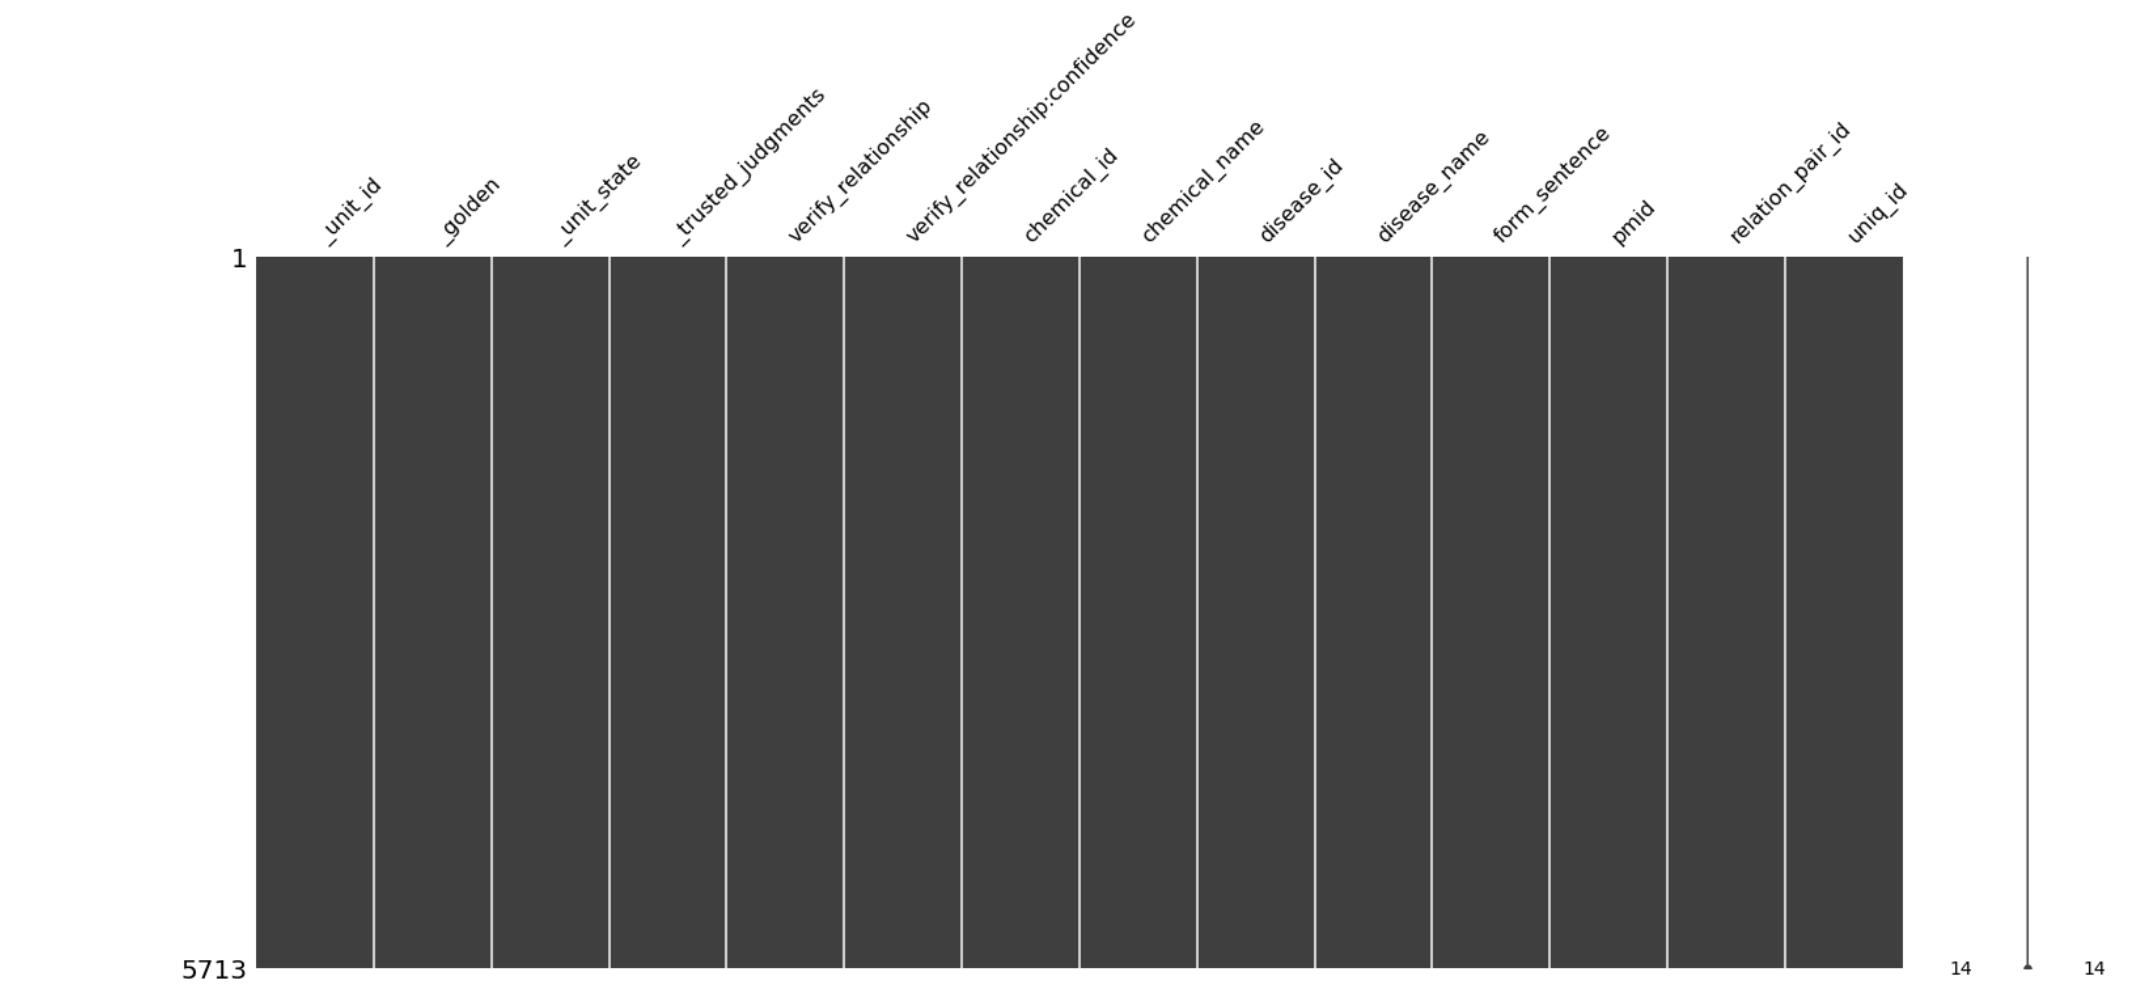
\includegraphics[width=.5\linewidth]{fig/data1.png}
        \label{fig:demo-fancy}}
\caption{\label{fig:demo}
}
\end{figure}



\subsection{Regular Expression}
The regular expression(re) module has been downloaded, removing the non-alpha numeric symbols in the chemical name and disease name columns.
\begin{figure}[h!t]
\centering
\subfigure[Before Drop Regular Expression]{\centering
    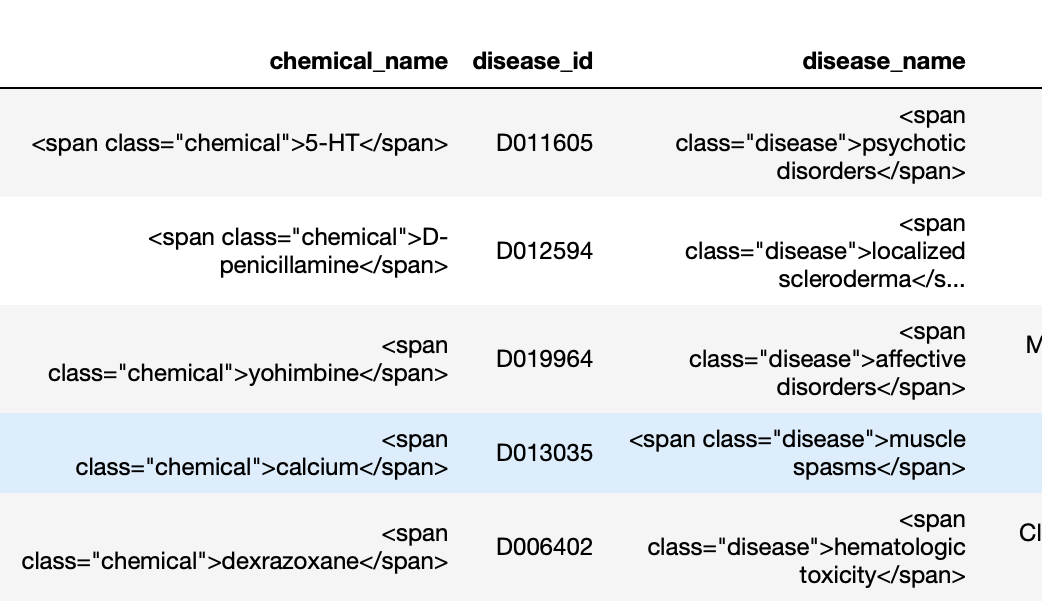
\includegraphics[width=.5\linewidth]{fig/before_exp.png}
        \label{fig:demo-standard}}
\subfigure[After Regular Expression]{\centering
    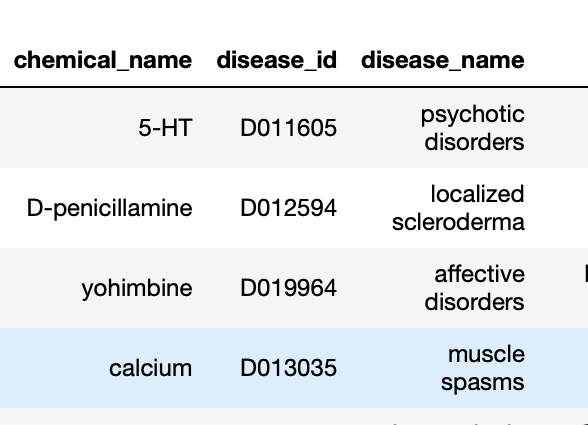
\includegraphics[width=.4\linewidth]{fig/after_exp.png}
        \label{fig:demo-fancy}}
\caption{\label{fig:demo}
}
\end{figure}






\subsection{Label Binarizer}
Our target field, the verify relationship values, were converted to binary value (0 or 1) using the sklearn labelBinarizer module from yes direct, yes-indirect and no-relation.
\subsection{Label Encoder}
Columns with categorical values were encoded as integers using the sklearn LabelEncoder method. A field pandas with a boolean value in its dataset is converted to integer value with the astype () method.
\subsection{Save Clean Data}
The dataframe (Figure 4) obtained as a result of data wrangling was saved in the csv file.
\subsection{Visualized Data}
The some fields in the dataframe were visualized using the seaborn library (Figure 5).

\begin{figure}[h!t]
\centering
{\centering
    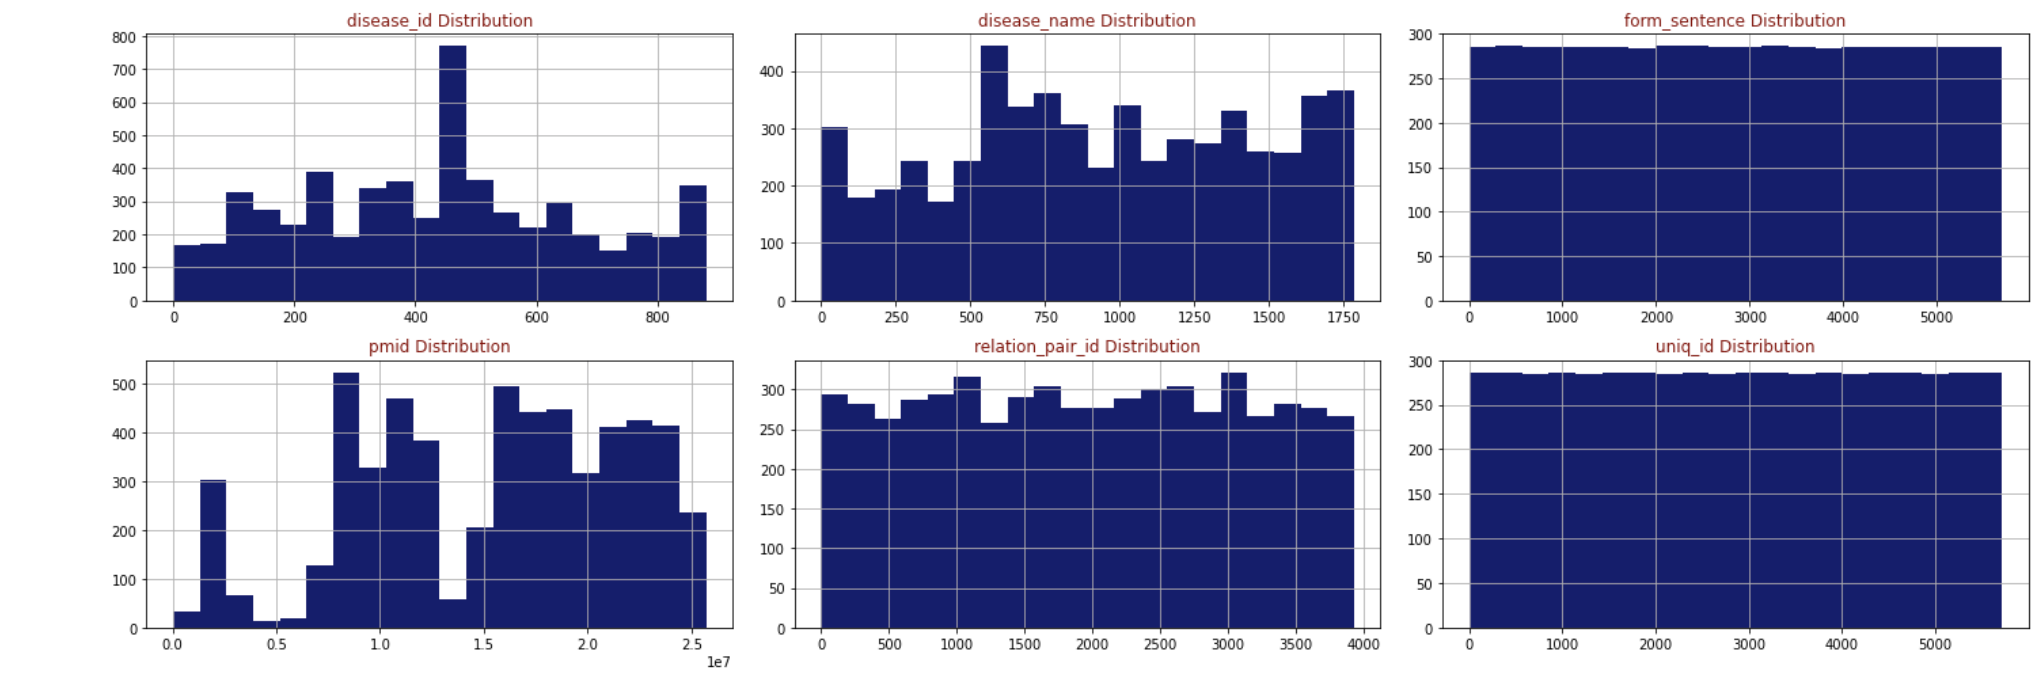
\includegraphics[width=14.1cm]{fig/visual.png}}        
\caption{Visual.}
\end{figure}



\section{The Model}

The cleaned dataset has been converted to the dataframe. The dataframe was divided into data and target groups, and the test was divided into 20 percent and the train 80 percent.

\begin{figure}[h!t]
\centering
{\centering
    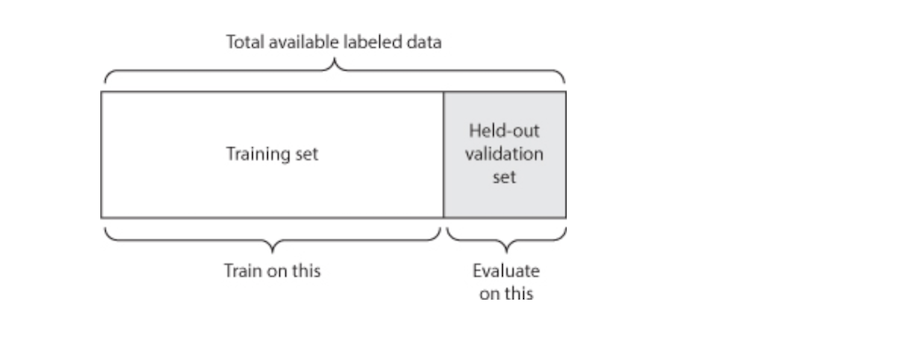
\includegraphics[width=10cm]{fig/model.png}}        
\caption{The illusturation of dataset }
\end{figure}



\subsection{Logistic Regression}
Logistic Regression is a regression method for classification. It is used to classify categorical or numerical data. It works only if the dependent variable, the result, could take 2 different values.
The data was trained using the logistic regression module from the sklearn library.
The training time of the data was monitored by making a stopwatch with the time module.
The score was observed using the test data.
\subsection{Support Vector Machines}
Support Vector Machine is a classification algorithm similar to Logistic Regression. Both try to find the best line that separates the two classes. The algorithm allows the line to be drawn to be adjusted in two classes so that it passes the furthest place to its elements. It is a classifier that takes no parameters (nonparametric).
The data was trained using the supported vector machines module from the sklearn library.
The training time of the data was monitored by making a stopwatch with the time module.
The score was observed using the test data.
\subsection{Perceptron}
Perceptron was inspired by the information processing of a single neural cell called a neuron. Persceptron is a linear classifier (binary). It is used in supervised learning. It helps to classify the given input data. Perceptron is often used to divide the data into two parts. Hence, it is also known as Linear Binary Classifier. The greater the number of data (tuples) the machine will train better. 
The data was trained using the perceptron module from the sklearn library.
The training time of the data was monitored by making a stopwatch with the time module.
The score was observed using the test data.
\section{Results}


In the field of data science, a confusion matrix, also known as an error matrix, is a specialized table layout, that allows the visualization of an algorithm's performance. I As the last step, the models were examined by using the confusion matrix.
Confusion matrix for Logistic Regression model:
\begin{figure}[h!t]
\centering
    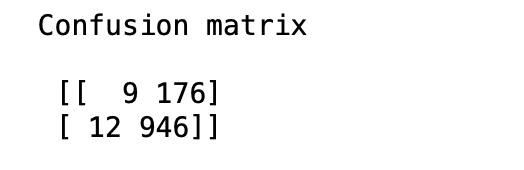
\includegraphics[width=.3\linewidth]{fig/conf_matrix.png}
\caption{\label{fig:dataset}
}
\end{figure}


The costs in classification plotted on the heatmap using the confusion matrix. 
Examine the confusion matrix for logistic regression:
\begin{figure}[h!t]
\centering
    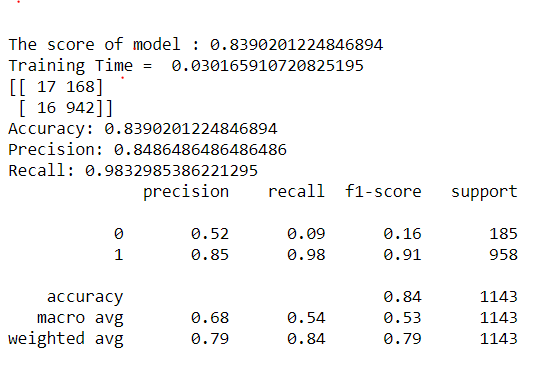
\includegraphics[width=.6\linewidth]{fig/log_regression.PNG}
\caption{\label{fig:dataset}
}
\end{figure}
The number of samples labeled 0 in the original is 186 ; 1s are 957(the sum for the lines). These numbers are named support.
The number of samples labeled 0 in the predicted dataset is 22; 1s are 1121 (the sum as columns).
Correct classifications are 963 (the sum of the diagonal).
Misclassifications are 180 (the sum of all numbers not on the diagonal).
Accuracy: The first measure we'll explore to evaluate the performance of the classifier is accuracy. Accuracy is the percentage of correct classifications over the total number of samples.
We can calculate this percentage over the confusion matrix as follows:
963/1157 = 0.83
Using Python, this becomes:
\begin{figure}[h!t]
\centering
    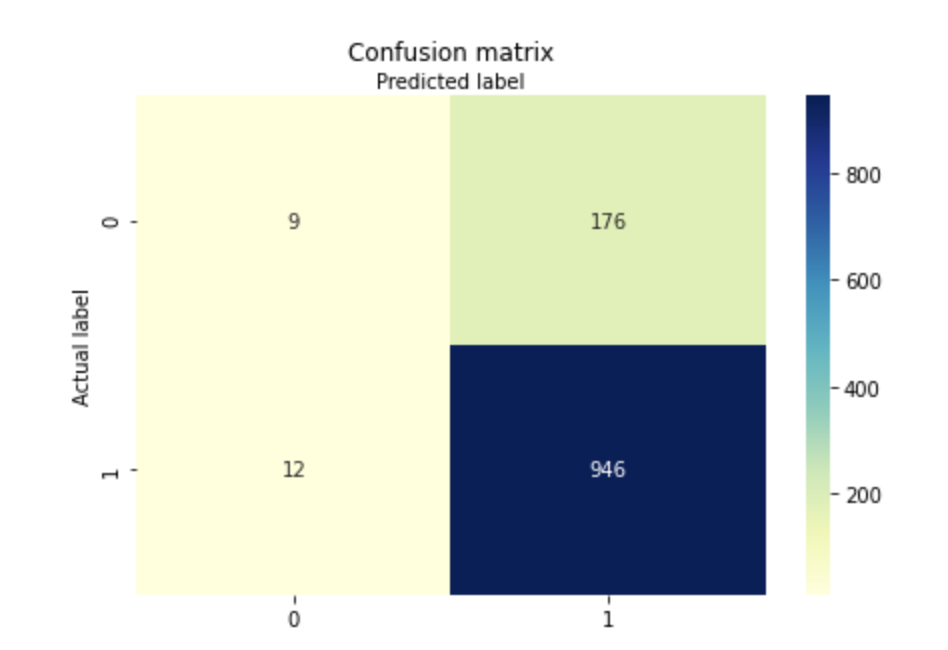
\includegraphics[width=.5\linewidth]{fig/heatmap.png}
\caption{\label{fig:dataset}
}
\end{figure}.
Examine the result for Support Vectores Machines:
\begin{figure}[h!t]
\centering
    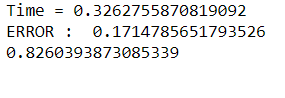
\includegraphics[width=.5\linewidth]{fig/svc.PNG}
\caption{\label{fig:dataset}
}
\end{figure}.

Examine the result for Perceptron:
\begin{figure}[h!t]
\centering
    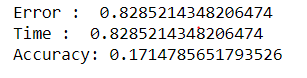
\includegraphics[width=.3\linewidth]{fig/perceptron.PNG}
\caption{\label{fig:dataset}
}
\end{figure}.


Screenshots are encouraged, but make sure they provide some useful insights. A two- or three-way comparison (perhaps with some particularly interesting part zoomed in) is typically a great way to present a single task. One example of a screenshot with caption is shown in figure \ref{fig:demo}. In case the assignment produces numbers, make sure you include them as this is typically a great way to compare, for example, performance. For example: \emph{In table X we show the area of different meshes using our implementation.}


\section{Conclusion}
In summary, classification is a process of categorizing a given set of data into classes. The problem framed, collect and clean the data, train the model, measure its performance, improve it by using some cost function, and then it is ready to deploy.
The sample in the dataset does not cover the whole population.
The dataset used in this project was first pre-processed and this cleaned dataset was classified according to three different learning algoritm (logistic regression, perceptron and support vectores machine).
The cost and time of the data set were measured and compared on different models.
As a result, the accuracy value of the dataset did not give the expected result. The reason for this is that the dataset used is not complex enough for this classification.
One of the most important issues in data science that significantly affects performance is that the amount of data is insufficient.
In other words, if we want to establish a better relationship between disease and chemicals, a data set with a further more data should be used.

\section{References}
1) O’Reilly Online Learning. 2020.Hands-On Machine Learning For Algorithmic Trading. [online] Available at: \url{https://learning.oreilly.com/library/view/hands-on-machine-learning/9781789346411/} [Accessed 28 December 2020].\\\\
2) Tarek Amr, Hands-On Machine Learning with \verb scikit-learn and Scientific Python \\\\
3) Subramanian, G., n.d. Python Data Science Cookbook. \\

\end{document}

